\documentclass{article}
\usepackage{fix-cm}
\usepackage[paperwidth=13.2in,paperheight=6.85in,margin=0.10in]{geometry}
\usepackage{amsmath}
\usepackage{tikz}
\usetikzlibrary{arrows.meta,positioning,calc}
\pagestyle{empty}

\begin{document}
\noindent
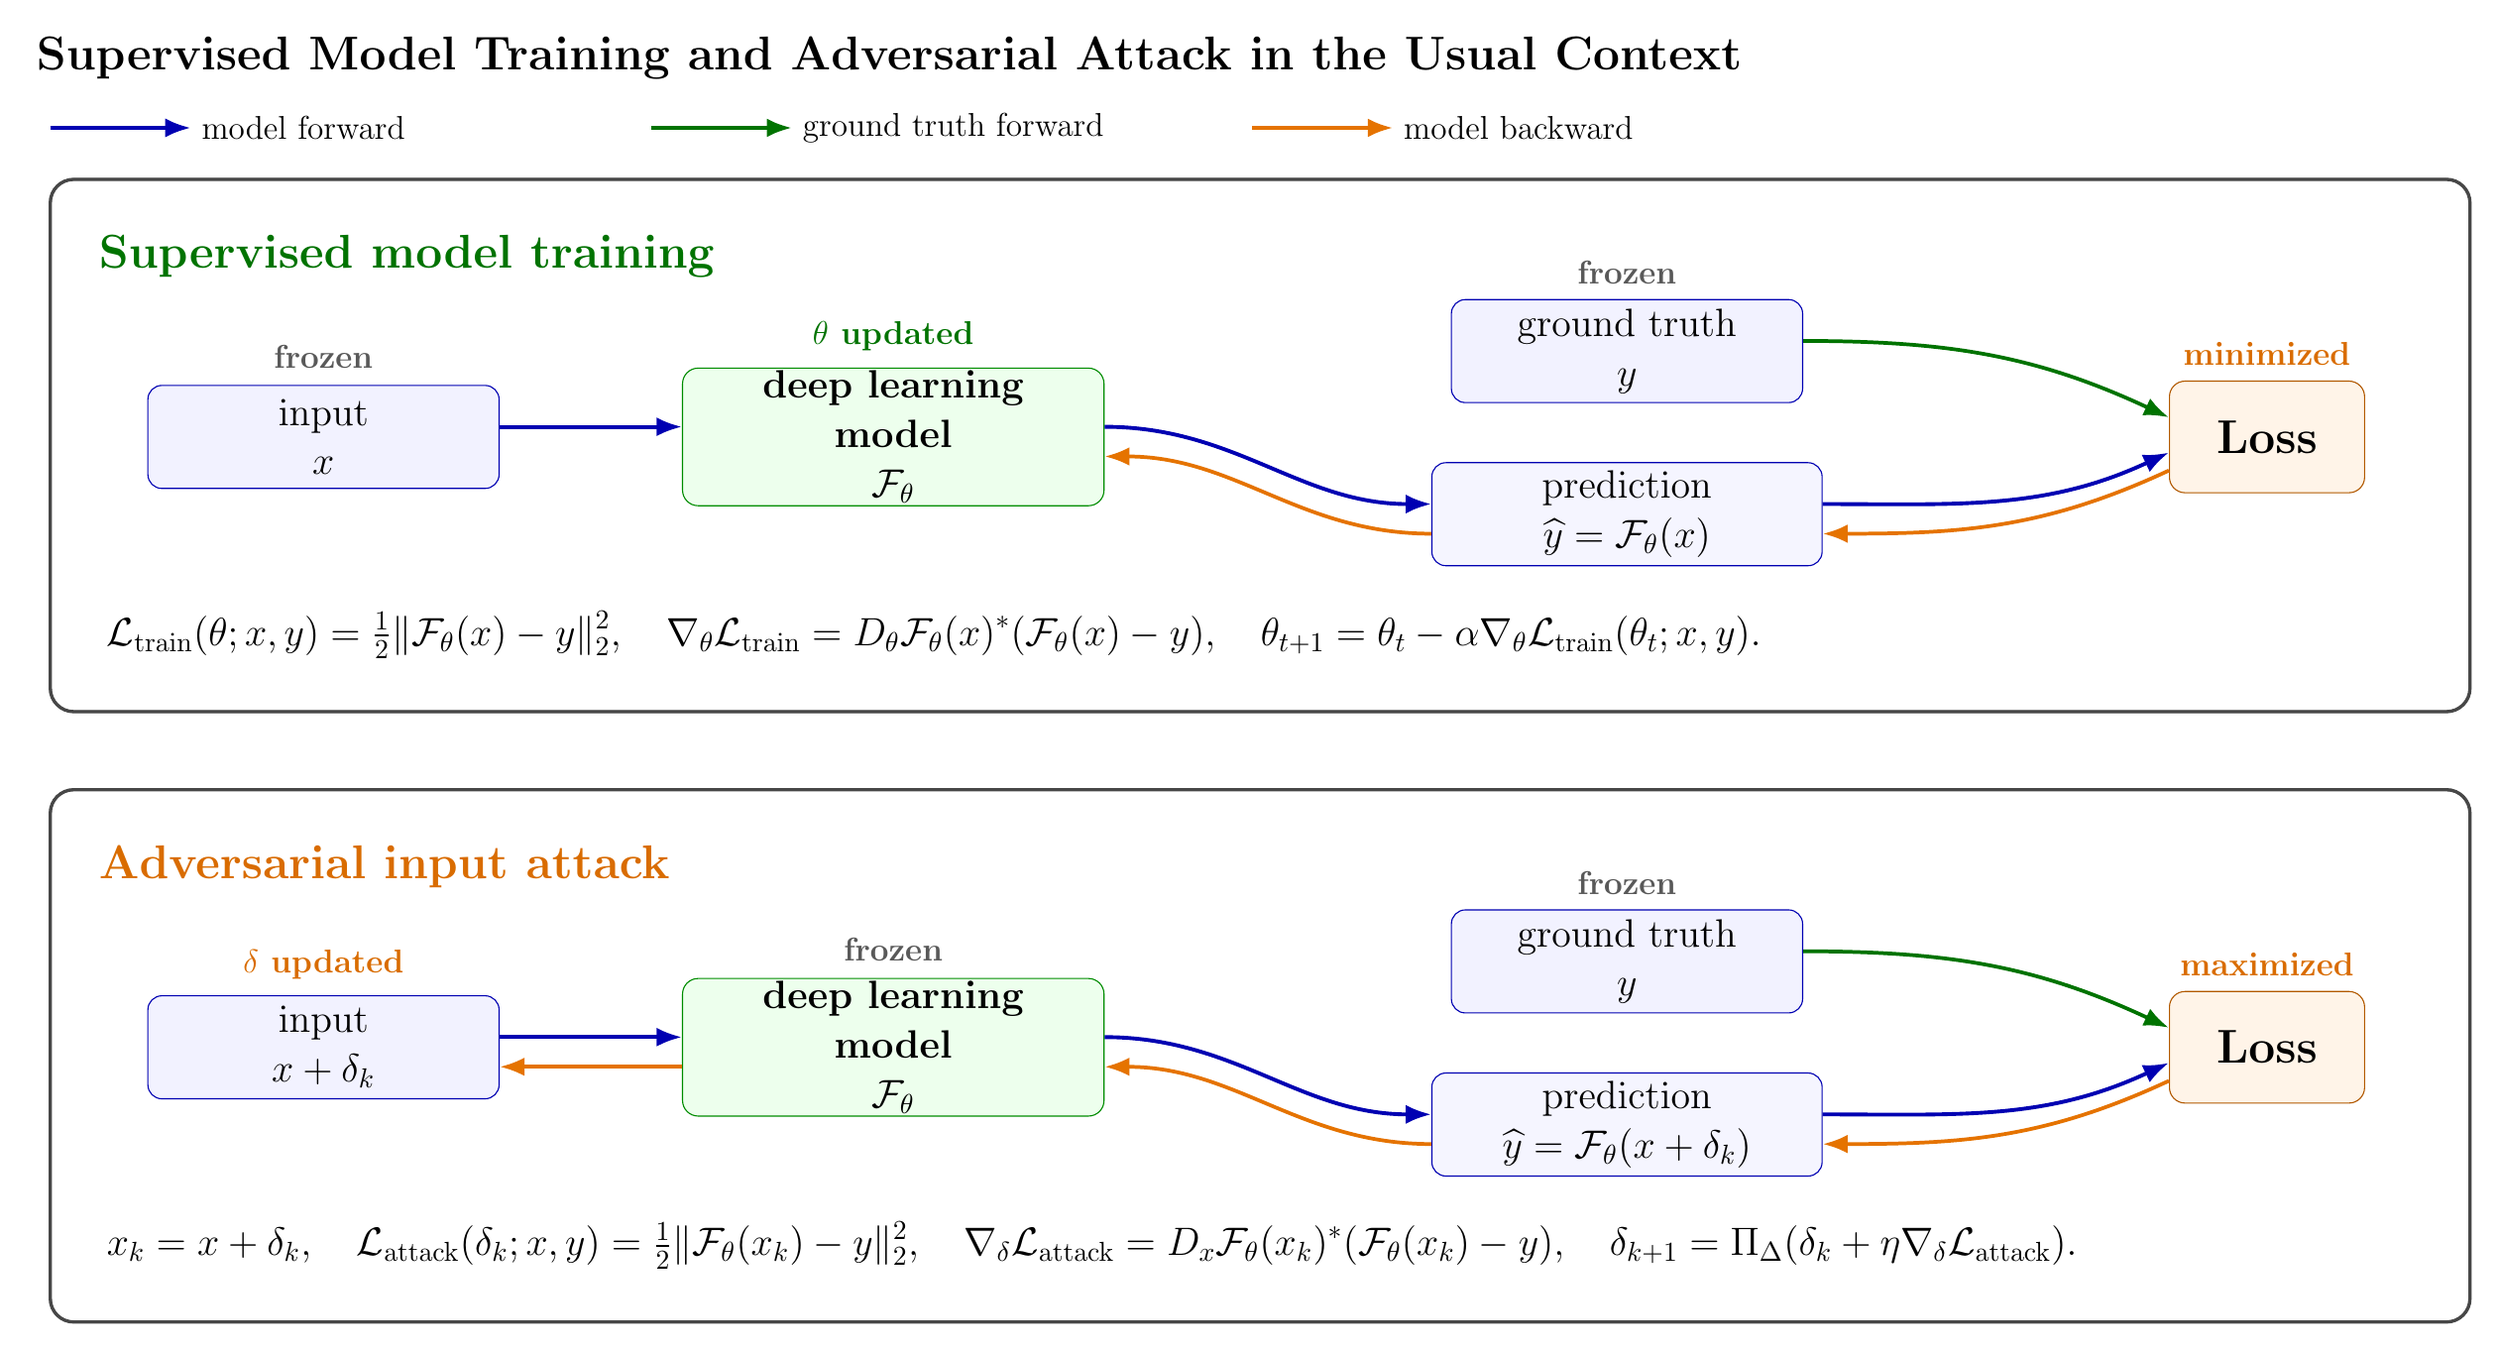
\begin{tikzpicture}[
  x=1mm,y=1mm,
  >=Latex,
  font=\sffamily,
  panel/.style={draw=black!55, rounded corners=3mm, line width=0.9pt, fill=white},
  box/.style={draw=black!60, rounded corners=1.6mm, fill=white, minimum height=13.2mm, align=center, font=\Large, inner ysep=1pt},
  gt/.style={draw=blue!70!black, rounded corners=1.8mm, fill=blue!5, minimum height=13.2mm, align=center, font=\Large, inner ysep=1pt},
  model/.style={draw=green!55!black, rounded corners=2mm, fill=green!7, minimum height=16.5mm, align=center, font=\Large\bfseries, inner ysep=1pt},
  pred/.style={draw=blue!70!black, rounded corners=1.8mm, fill=blue!4, minimum height=13.2mm, align=center, font=\Large, inner ysep=1pt},
  loss/.style={draw=orange!70!black, rounded corners=2mm, fill=orange!9, minimum width=25mm, minimum height=14.3mm, align=center, font=\LARGE\bfseries, inner ysep=1pt},
  label/.style={font=\LARGE\bfseries, anchor=west},
  formula/.style={font=\Large, anchor=south west, align=left},
  note/.style={font=\large, text=black!65, align=center},
  smallnote/.style={font=\large\bfseries, text=black!65, align=center, anchor=south},
  action/.style={font=\large\bfseries, align=center, anchor=south},
  fwd/.style={->, draw=blue!70!black, line width=1.4pt},
  gtfwd/.style={->, draw=green!45!black, line width=1.35pt},
  bwd/.style={->, draw=orange!90!black, line width=1.35pt},
  fixed/.style={draw=black!45, line width=0.9pt, dashed}
]

% Title and legend
\node[font=\LARGE\bfseries, anchor=west] at (5,168)
  {Supervised Model Training and Adversarial Attack in the Usual Context};
\draw[fwd] (8,159) -- ++(18,0) node[right, black, font=\large] {model forward};
\draw[gtfwd] (85,159) -- ++(18,0) node[right, black, font=\large] {ground truth forward};
\draw[bwd] (162,159) -- ++(18,0) node[right, black, font=\large] {model backward};

% ================= Panel 1: training =================
\begin{scope}[shift={(0,84.2)}]
  \draw[panel] (8,0) rectangle (318,68.2);
  \node[label, text=green!45!black] at (13,58.3) {Supervised model training};
  \node[formula] at (14,5.5)
    {$\displaystyle \mathcal L_{\mathrm{train}}(\theta;x,y)=\tfrac12\|\mathcal F_\theta(x)-y\|_2^2,\quad \nabla_\theta\mathcal L_{\mathrm{train}}=D_\theta\mathcal F_\theta(x)^*(\mathcal F_\theta(x)-y),\quad \theta_{t+1}=\theta_t-\alpha\nabla_\theta\mathcal L_{\mathrm{train}}(\theta_t;x,y).$};

  \node[gt, minimum width=45mm] (xin) at (43,35.2) {input\\$x$};
  \node[model, minimum width=54mm] (model) at (116,35.2) {deep learning\\model\\$\mathcal F_\theta$};
  \node[pred, minimum width=50mm] (ypred) at (210,25.3) {prediction\\$\widehat y=\mathcal F_\theta(x)$};
  \node[gt, minimum width=45mm] (ygt) at (210,46.2) {ground truth\\$y$};
  \node[loss] (loss) at (292,35.2) {Loss};

  \node[smallnote] at (43,42.7) {frozen};
  \node[smallnote, text=green!45!black] at (116,45.0) {$\theta$ updated};
  \node[smallnote] at (210,53.5) {frozen};
  \node[action, text=orange!85!black] at (292,43.1) {minimized};

  \draw[fwd] ([yshift=1.3mm]xin.east) -- ([yshift=1.3mm]model.west);
  \draw[fwd] ([yshift=1.3mm]model.east) to[out=0,in=180] ([yshift=1.3mm]ypred.west);
  \draw[gtfwd] ([yshift=1.3mm]ygt.east) to[out=0,in=155] ([yshift=2.5mm]loss.west);
  \draw[fwd] ([yshift=1.3mm]ypred.east) to[out=0,in=205] ([yshift=-2.0mm]loss.west);

  \draw[bwd] ([yshift=-4.3mm]loss.west) to[out=205,in=0] ([yshift=-2.5mm]ypred.east);
  \draw[bwd] ([yshift=-2.5mm]ypred.west) to[out=180,in=0] ([yshift=-2.5mm]model.east);
\end{scope}

% ================= Panel 2: attack =================
\begin{scope}[shift={(0,6)}]
  \draw[panel] (8,0) rectangle (318,68.2);
  \node[label, text=orange!85!black] at (13,58.3) {Adversarial input attack};
  \node[formula] at (14,5.5)
    {$\displaystyle x_k=x+\delta_k,\quad \mathcal L_{\mathrm{attack}}(\delta_k;x,y)=\tfrac12\|\mathcal F_\theta(x_k)-y\|_2^2,\quad \nabla_\delta\mathcal L_{\mathrm{attack}}=D_x\mathcal F_\theta(x_k)^*(\mathcal F_\theta(x_k)-y),\quad \delta_{k+1}=\Pi_\Delta(\delta_k+\eta\nabla_\delta\mathcal L_{\mathrm{attack}}).$};

  \node[gt, minimum width=45mm] (xin) at (43,35.2) {input\\$x+\delta_k$};
  \node[model, minimum width=54mm] (model) at (116,35.2) {deep learning\\model\\$\mathcal F_\theta$};
  \node[pred, minimum width=50mm] (ypred) at (210,25.3) {prediction\\$\widehat y=\mathcal F_\theta(x+\delta_k)$};
  \node[gt, minimum width=45mm] (ygt) at (210,46.2) {ground truth\\$y$};
  \node[loss] (loss) at (292,35.2) {Loss};

  \node[smallnote, text=orange!85!black] at (43,42.7) {$\delta$ updated};
  \node[smallnote] at (116,45.0) {frozen};
  \node[smallnote] at (210,53.5) {frozen};
  \node[action, text=orange!85!black] at (292,43.1) {maximized};

  \draw[fwd] ([yshift=1.3mm]xin.east) -- ([yshift=1.3mm]model.west);
  \draw[fwd] ([yshift=1.3mm]model.east) to[out=0,in=180] ([yshift=1.3mm]ypred.west);
  \draw[gtfwd] ([yshift=1.3mm]ygt.east) to[out=0,in=155] ([yshift=2.5mm]loss.west);
  \draw[fwd] ([yshift=1.3mm]ypred.east) to[out=0,in=205] ([yshift=-2.0mm]loss.west);

  \draw[bwd] ([yshift=-4.3mm]loss.west) to[out=205,in=0] ([yshift=-2.5mm]ypred.east);
  \draw[bwd] ([yshift=-2.5mm]ypred.west) to[out=180,in=0] ([yshift=-2.5mm]model.east);
  \draw[bwd] ([yshift=-2.5mm]model.west) to[out=180,in=0] ([yshift=-2.5mm]xin.east);
\end{scope}

% Redraw panel borders on the foreground so the left edges remain solid in PDF/PNG output.
\draw[draw=black!72, rounded corners=3mm, line width=1.2pt, line join=round]
  (8,84.2) rectangle (318,152.4);
\draw[draw=black!72, line width=1.2pt, line cap=round] (8,88.2) -- (8,148.4);
\draw[draw=black!72, rounded corners=3mm, line width=1.2pt, line join=round]
  (8,6) rectangle (318,74.2);
\draw[draw=black!72, line width=1.2pt, line cap=round] (8,10) -- (8,70.2);

\end{tikzpicture}
\end{document}
